\documentclass[12pt]{beamer}

\usepackage[size = custom, width = 140, height = 73, scale = 1.75]{beamerposter}

\usefonttheme{serif}

\usepackage[english]{babel}
\usepackage[utf8x]{inputenc}
\usepackage[T1]{fontenc}
\usepackage{lmodern}
\usepackage{indentfirst}
\usepackage{ragged2e}
\usepackage[]{natbib} 
\usepackage{graphicx}
\usepackage{animate}
\usepackage{color}
\usepackage{colortbl}
\usepackage{xr}

% For 'InkScape' integration
\usepackage{import}
\usepackage{xifthen}
\usepackage{pdfpages}
\usepackage{transparent}

\setbeamertemplate{navigation symbols}{}
\setbeamertemplate{caption}[numbered]

\definecolor{title-bg}{RGB}{240, 240, 240}
\definecolor{title-fg}{RGB}{128, 113, 93}
\definecolor{my-red}{RGB}{254, 132, 135}
\definecolor{my-blue}{RGB}{59, 180, 252}
\definecolor{my-green}{RGB}{125, 221, 149}
\definecolor{titles}{RGB}{0, 166, 160}
\setbeamercolor{block title}{fg = title-fg, bg = title-bg}
\setbeamercolor{header-color}{fg = title-fg, bg = title-bg}

\setbeamertemplate{headline}{%
\begin{beamercolorbox}[wd=1.00\textwidth]{header-color}
	\begin{columns}[T]
		\begin{column}{0.235\textwidth}
			
\includegraphics[width=1.15\linewidth]{Images/KAUST_logo} 
		\end{column}
		\begin{column}{0.630\textwidth}
			\vspace{32pt}
			\begin{beamercolorbox}[wd=1.00\textwidth]{header-color}	
			{\Large Extended Excess Hazard Model for Spatially Dependent Survival Data with Applications to Cancer Research \par} \vspace{15pt}
			
			{\normalsize
				André Victor Ribeiro Amaral${\phantom{|}}^{1, \star}$, 
				Francisco Javier Rubio${\phantom{|}}^{2}$,  and 
				Paula Moraga${\phantom{|}}^{1}$
			}	\vspace{12pt}
		
			{\footnotesize
			${}^{1}\hspace{8pt}$Computer, Electrical and Mathematical Sciences and Engineering Division, King Abdullah University of Science and Technology (KAUST).  \\ \vspace{3pt}
			${}^{2}\hspace{8pt}$Department of Statistical Science, University College London (UCL).  \\ \vspace{6pt}
			${}^{\star}$ E-mail: \texttt{andre.ribeiroamaral@kaust.edu.sa}
			}
			\end{beamercolorbox}
			\vspace{3pt}
		\end{column}
		\begin{column}{0.15\textwidth}
		\vspace{25pt}
		
\includegraphics[width=0.85\linewidth]{Images/GeoHealth_logo}
		\end{column}
	\end{columns}
\end{beamercolorbox}
}
\setbeamertemplate{footline}{}

\begin{document}
	\begin{frame}[t]
		\vspace{-36pt}
		\begin{columns}[t]
			%======================================== FIRST COLUMN ========================================
			\begin{column}{0.30\textwidth} \justifying % FIRST COLUMN
			\begin{block}{\Large 1 Introduction} \justifying \vspace{12pt}				
			
			In the relative survival framework, it is assumed an additive decomposition of the hazard function $h(\cdot)$ into two components, namely the hazard associated to other causes of death $h_{\text{O}}(\cdot)$, and the hazard associated to the study cancer $h_{\text{E}}(\cdot)$. That is, given covariates,
			\begin{align} \label{eq:main-haz}
				h(t; \mathbf{x}) = h_{\text{O}}(\text{age} + t) + h_{\text{E}}(t; \mathbf{x}),~ t \geq 0,
			\end{align}
			where ``age'' is the patient age when diagnosed, and $\mathbf{x}$ is a vector of risk factors. Also, as $h_{\text{O}}(\text{age} + t)$ is typically unknown in practice, it is common practice to approximate it by the population hazard $h_{\text{P}}(\text{age} + t; \mathbf{z})$, obtained from the life tables, such that $\mathbf{z} \subseteq \mathbf{x}$.
			
			\vspace{12pt}
			
			However, it is known that cancer registry data may present a spatially dependent structure, as patients from adjacent neighborhoods are likely to share environmental and social-economical factors.
				
			\vspace{18pt}
			
			\end{block}
			
			\begin{block}{\Large 2 Modeling Approach} \justifying \vspace{12pt}				
								
				Let $t_{ij}$ be the observed survival times, such that $i = 1, \cdots, r$ indicates the region and $j = 1, \cdots, n_i$ denotes the individuals. Then,
				\begin{align} \label{eq:exc-haz}
					h_{\text{E}}(t_{ij}; \mathbf{x}_{ij}, \tilde{u}_i, u_i) = h_0(t_{ij} \exp\{\tilde{\mathbf{x}}_{ij}^{\top} \boldsymbol{\alpha} + \tilde{u}_i\}) \exp\{\mathbf{x}_{ij}^{\top} \boldsymbol{\beta} + u_i\},
				\end{align}
				where $h_0(\cdot)$ is the baseline function modeled in a parametric manner.
				
				\vspace{12pt}
				
				Model \ref{eq:exc-haz}---Relative Survival Mixed-effects General Hazard (RS-MEGH) model---generalizes the following approaches
				
				\begin{table}[]
					%\resizebox{\textwidth}{!}{%
					\caption{\justifying Eight simpler models based on the Relative Survival Mixed-effects General Hazard (RS-MEGH) approach.}
					\label{tab:models}
					\begin{tabular}{l | c | l | c }
						Name & Description & Name & Description  \\ \hline 
						RS-MEGH-I &  $\tilde{\mathbf{u}} = \mathbf{0}$& RS-GH & $\tilde{\mathbf{u}} = \mathbf{u} = \mathbf{0}$ \\
						RS-MEGH-II &  $\tilde{\mathbf{u}} = \mathbf{u}$& RS-PH & $\tilde{\mathbf{u}} = \mathbf{u} = \mathbf{0}, \boldsymbol{\alpha} = \mathbf{0}$ \\
						RS-MEPH &  $\tilde{\mathbf{u}} = \mathbf{0}, \boldsymbol{\alpha} = \mathbf{0}$& RS-AFT & $\tilde{\mathbf{u}} = \mathbf{u} = \mathbf{0}, \boldsymbol{\alpha} = \boldsymbol{\beta}$ \\
						RS-MEAFT &  $\tilde{\mathbf{u}} = \mathbf{u}, \boldsymbol{\alpha} = \boldsymbol{\beta}$& RS-AH&  $\tilde{\mathbf{u}} = \mathbf{u} = \mathbf{0}, \boldsymbol{\beta} = \mathbf{0}$ \\
					\end{tabular}%
					%}
				\end{table}
				
				\vspace{18pt}
				
			\end{block}
			
			\end{column}
		
			%======================================== SECOND COLUMN ========================================
			\begin{column}{0.30\textwidth} \justifying % SECOND COLUMN
			
			{\large \textcolor{title-fg}{2.1 Spatial Model}} \vspace{18pt}
			
			We want to model $\tilde{\mathbf{u}}$ and $\mathbf{u}$ in such a way that these random effects smooth the data according to the observed neighborhood structure. 
			
			\vspace{18pt}
			
			{\textcolor{title-fg}{2.1.1 ICAR Model}} \vspace{18pt}
			
			For the Intrinsic Conditional Autoregressive (ICAR) model \citep{besag:1974}, the conditional distribution of $u_i$ given $u_j$, such that $j\hspace{-6pt}\neq\hspace{-6pt}i$ (not. $\mathbf{u}_{-i}$), is
			\begin{align*} 
				\pi(u_i | \mathbf{u}_{-i}) = \text{Normal}\left(\frac{\displaystyle\raisebox{-18pt}{\scalebox{3.2}{\ensuremath{\sum}}}_{k \in \Lambda_{i}} u_k}{\lambda_{i}}, \frac{\sigma_i^2}{\lambda_i}\right),
			\end{align*}
			where $\Lambda_i$ and $\lambda_i$ correspond to the neighbors and the number of neighbors of region $i$, \hspace{-6pt}respectively.\hspace{-6pt} The joint model can be written as
			\begin{align} \label{eq:pairwise}
				\pi(\mathbf{u}) \propto \tau_u^{\frac{r - 1}{2}}\exp\left\{-\frac{\tau_u}{2}\displaystyle\raisebox{-18pt}{\scalebox{3.2}{\ensuremath{\sum}}}_{i \sim j} (u_i - u_j) ^ 2\right\},
			\end{align}
			where $\tau_u$ is the precision parameter. From Equation \eqref{eq:pairwise}, $\displaystyle\raisebox{-18pt}{\scalebox{3.2}{\ensuremath{\sum}}}_{\text{all } i} u_i = 0$.
			
			\vspace{18pt}
						
			{\textcolor{title-fg}{2.1.2 BYM2 Model}} \vspace{18pt}
			
			For the Besag-York-Mollié (BYM2) model \citep{besag:1991}, the unstructured and structured random effects can be written as
			\begin{align*} 
				\mathbf{v} + \mathbf{u} = \sigma(\sqrt{1 - \rho} \mathbf{v}^{\star} + \sqrt{\rho}\mathbf{u}^{\star}),
			\end{align*}
			where $\sigma$ represents the overall standard deviation, $\rho \in [0, 1]$, $\mathbf{v}^{\star} \sim \text{Normal}(\mathbf{0}, I_r)$, and $\mathbf{u}^{\star}$ is the scaled ICAR model.
			
			\vspace{18pt}
			
			\begin{block}{\Large 3 Estimation procedure} \justifying \vspace{12pt}				
				
			Let $\mathcal{D} = \{(t_{ij}, \delta_{ij}, \mathbf{x}_{ij}, \mathbf{z}_{ij}); i = 1, \cdots, r, \text{ and } j = 1, \cdots, n_i\}$ be the observed data. In that case, the likelihood function for the vector of unknown parameters $\boldsymbol{\xi}$ can be written as proportional to
			\begin{align*}
				\displaystyle\raisebox{-18pt}{\scalebox{3.2}{\ensuremath{\prod}}}_{i = 1}^{r}\displaystyle\raisebox{-18pt}{\scalebox{3.2}{\ensuremath{\prod}}}_{j = 1}^{n_i} \left\{h_{\text{P}}(\text{age}_{ij} + t_{ij}; \mathbf{z}_{ij}) + h_{\text{E}}(t_{ij}; \mathbf{x}_{ij}, \tilde{u}_i, u_i)\right\}^{\delta_{ij}} \times \\ 
				\times \exp\{-H_{\text{E}}(t_{ij}; \textbf{x}_{ij}, \tilde{u}_i, u_i)\},
			\end{align*}
			where $h_{\text{P}}(\text{age}_{ij} + t_{ij}; \mathbf{z}_{ij})$ is previously obtained from the life tables. 
				
				\vspace{18pt}
				
			\end{block}
			
			\vspace{18pt}
			
			\end{column}
		
			%======================================== THIRD COLUMN ========================================
			\begin{column}{0.30\textwidth} \justifying % THIRD COLUMN
		
			\begin{block}{\Large 4 Case Study} \justifying \vspace{12pt}				
				
		We will analyze a data set that contains survival information about $n = 1,043$ patients diagnosed with acute myeloid leukemia between 1982 and 1998 in the 24 areas in the North West region of the UK.	
		
		\vspace{12pt}
		
		After fitting possible model combinations, the highest ranked approach was the RS-MEGH (LN ICAR). The results are based on it.
		
		\vspace{12pt}
		
		To compare the areas, we will compute the ``net survival'' as follows
		\begin{align*} 
			S_{\text{N}}(t_{i}) = (n_i)^{-1}\displaystyle\raisebox{-26pt}{\scalebox{4.5}{\ensuremath{\sum}}}_{j=1}^{n_i}\exp\{-\displaystyle\raisebox{-26pt}{\scalebox{4.5}{\ensuremath{\int}}}_{0}^{t_{ij}} h_{\text{E}}(\ell; \textbf{x}_{ij}, \tilde{u}_i, u_i) d\ell\}, ~\forall i.
		\end{align*}
	
		Figure \ref{fig:map} shows the estimated net survival function $S_{N}(t_i)$, $\forall i$, where $t_i = 1$ (years), such that the data was stratified by deprivation level.
	
		\begin{figure}[!ht]
			\centering
			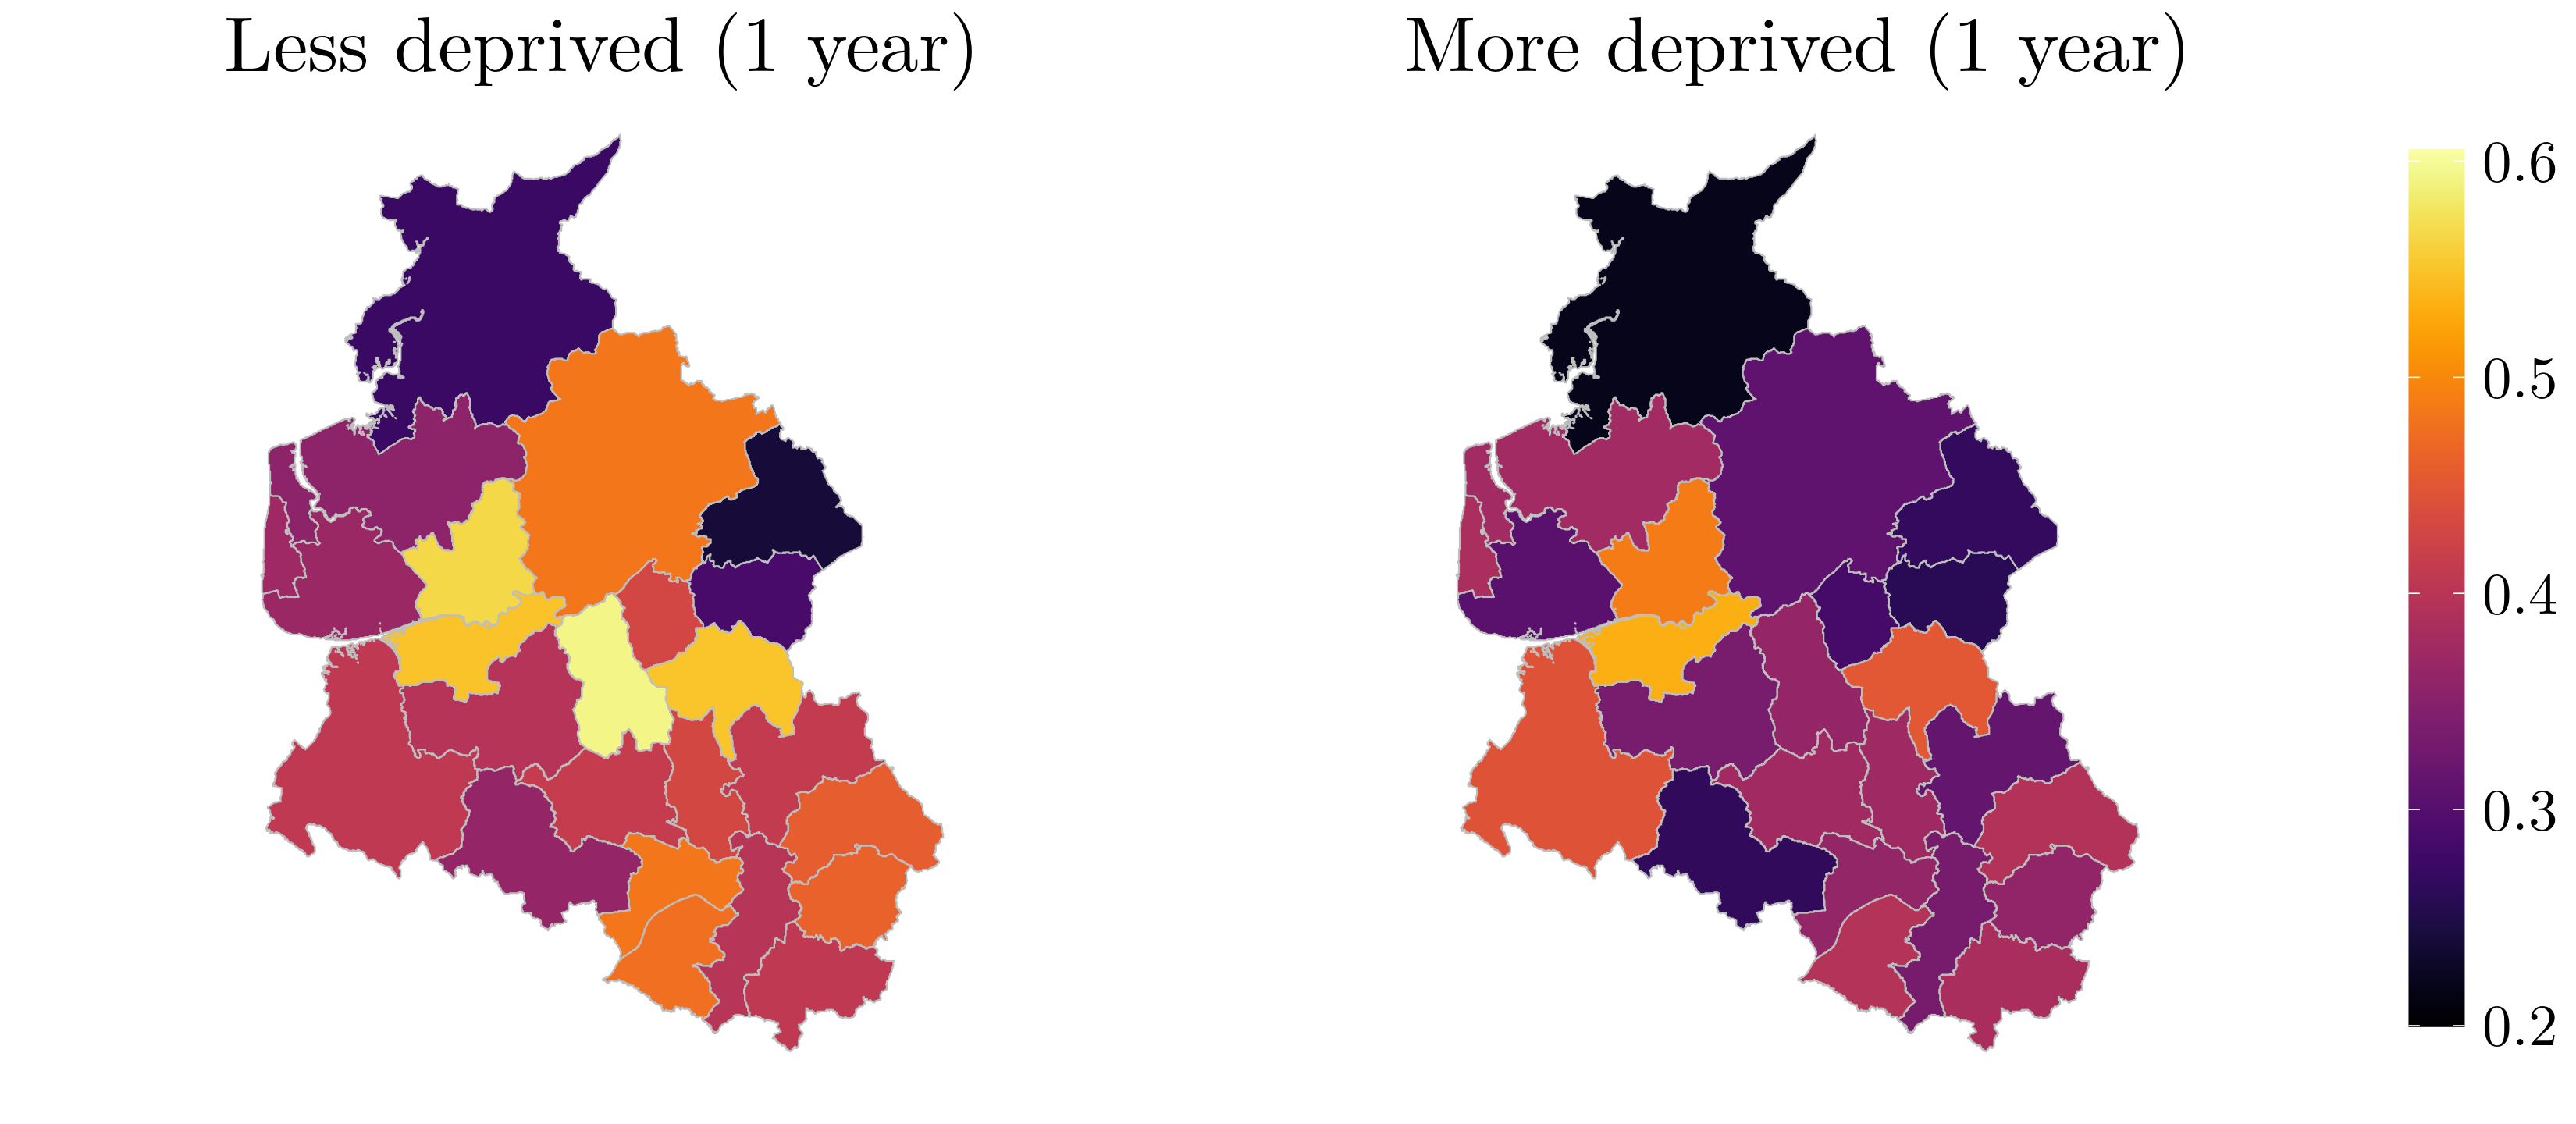
\includegraphics[width = 0.775\textwidth]{Images/map_poster}
			\caption{\justifying Estimated net survival function, after 1 year, for two groups of patients.}
			\label{fig:map}
		\end{figure}	
				
		In conclusion, it seems that, based on the analyzed data, the patients' location contribute to their chances of surviving when diagnosed with leukemia. Therefore, modeling the spatially dependent random effects might be important to understand how these individuals are treated in different manners across the North West region of the UK.

		\vspace{18pt}
				
		\end{block}
			
		{\textcolor{title-fg}{References}} \vspace{18pt}
		\scriptsize
		\bibliographystyle{plain}
		\bibliography{References/References}
					
		\end{column}
		\end{columns}
	\end{frame}


\end{document}
